\section{AI 에이전트 아키텍처}

본 절에서는 실제 설계 및 구현된 다중 에이전트 시스템의 구체적인 아키텍처와 동작 메커니즘을 서술한다. 본 시스템은 도메인별로 특화된 3종의 공격 (RED) 계획 에이전트, 전체 교전을 조율하는 1종의 아레나 오케스트레이터 (arena orchestrator), 그리고 모든 도메인에 걸쳐 방어를 수행하는 1종의 단일 공유 방어 (BLUE) 커맨더로 구성된다. 이하의 내용은 \texttt{src/agents/} 및 \texttt{src/defenses/} 디렉터리의 실제 구현 코드와 정확히 대응하며, 인용된 모든 정량적 수치는 시뮬레이션 전용 (sim-only) 환경에서 실측된 실행 로그를 엄밀한 근거로 삼는다.

\subsection{아키텍처 개요: 다중 도메인 RED, 오케스트레이터, 단일 공유 BLUE}

\begin{figure}[t!]
\centering
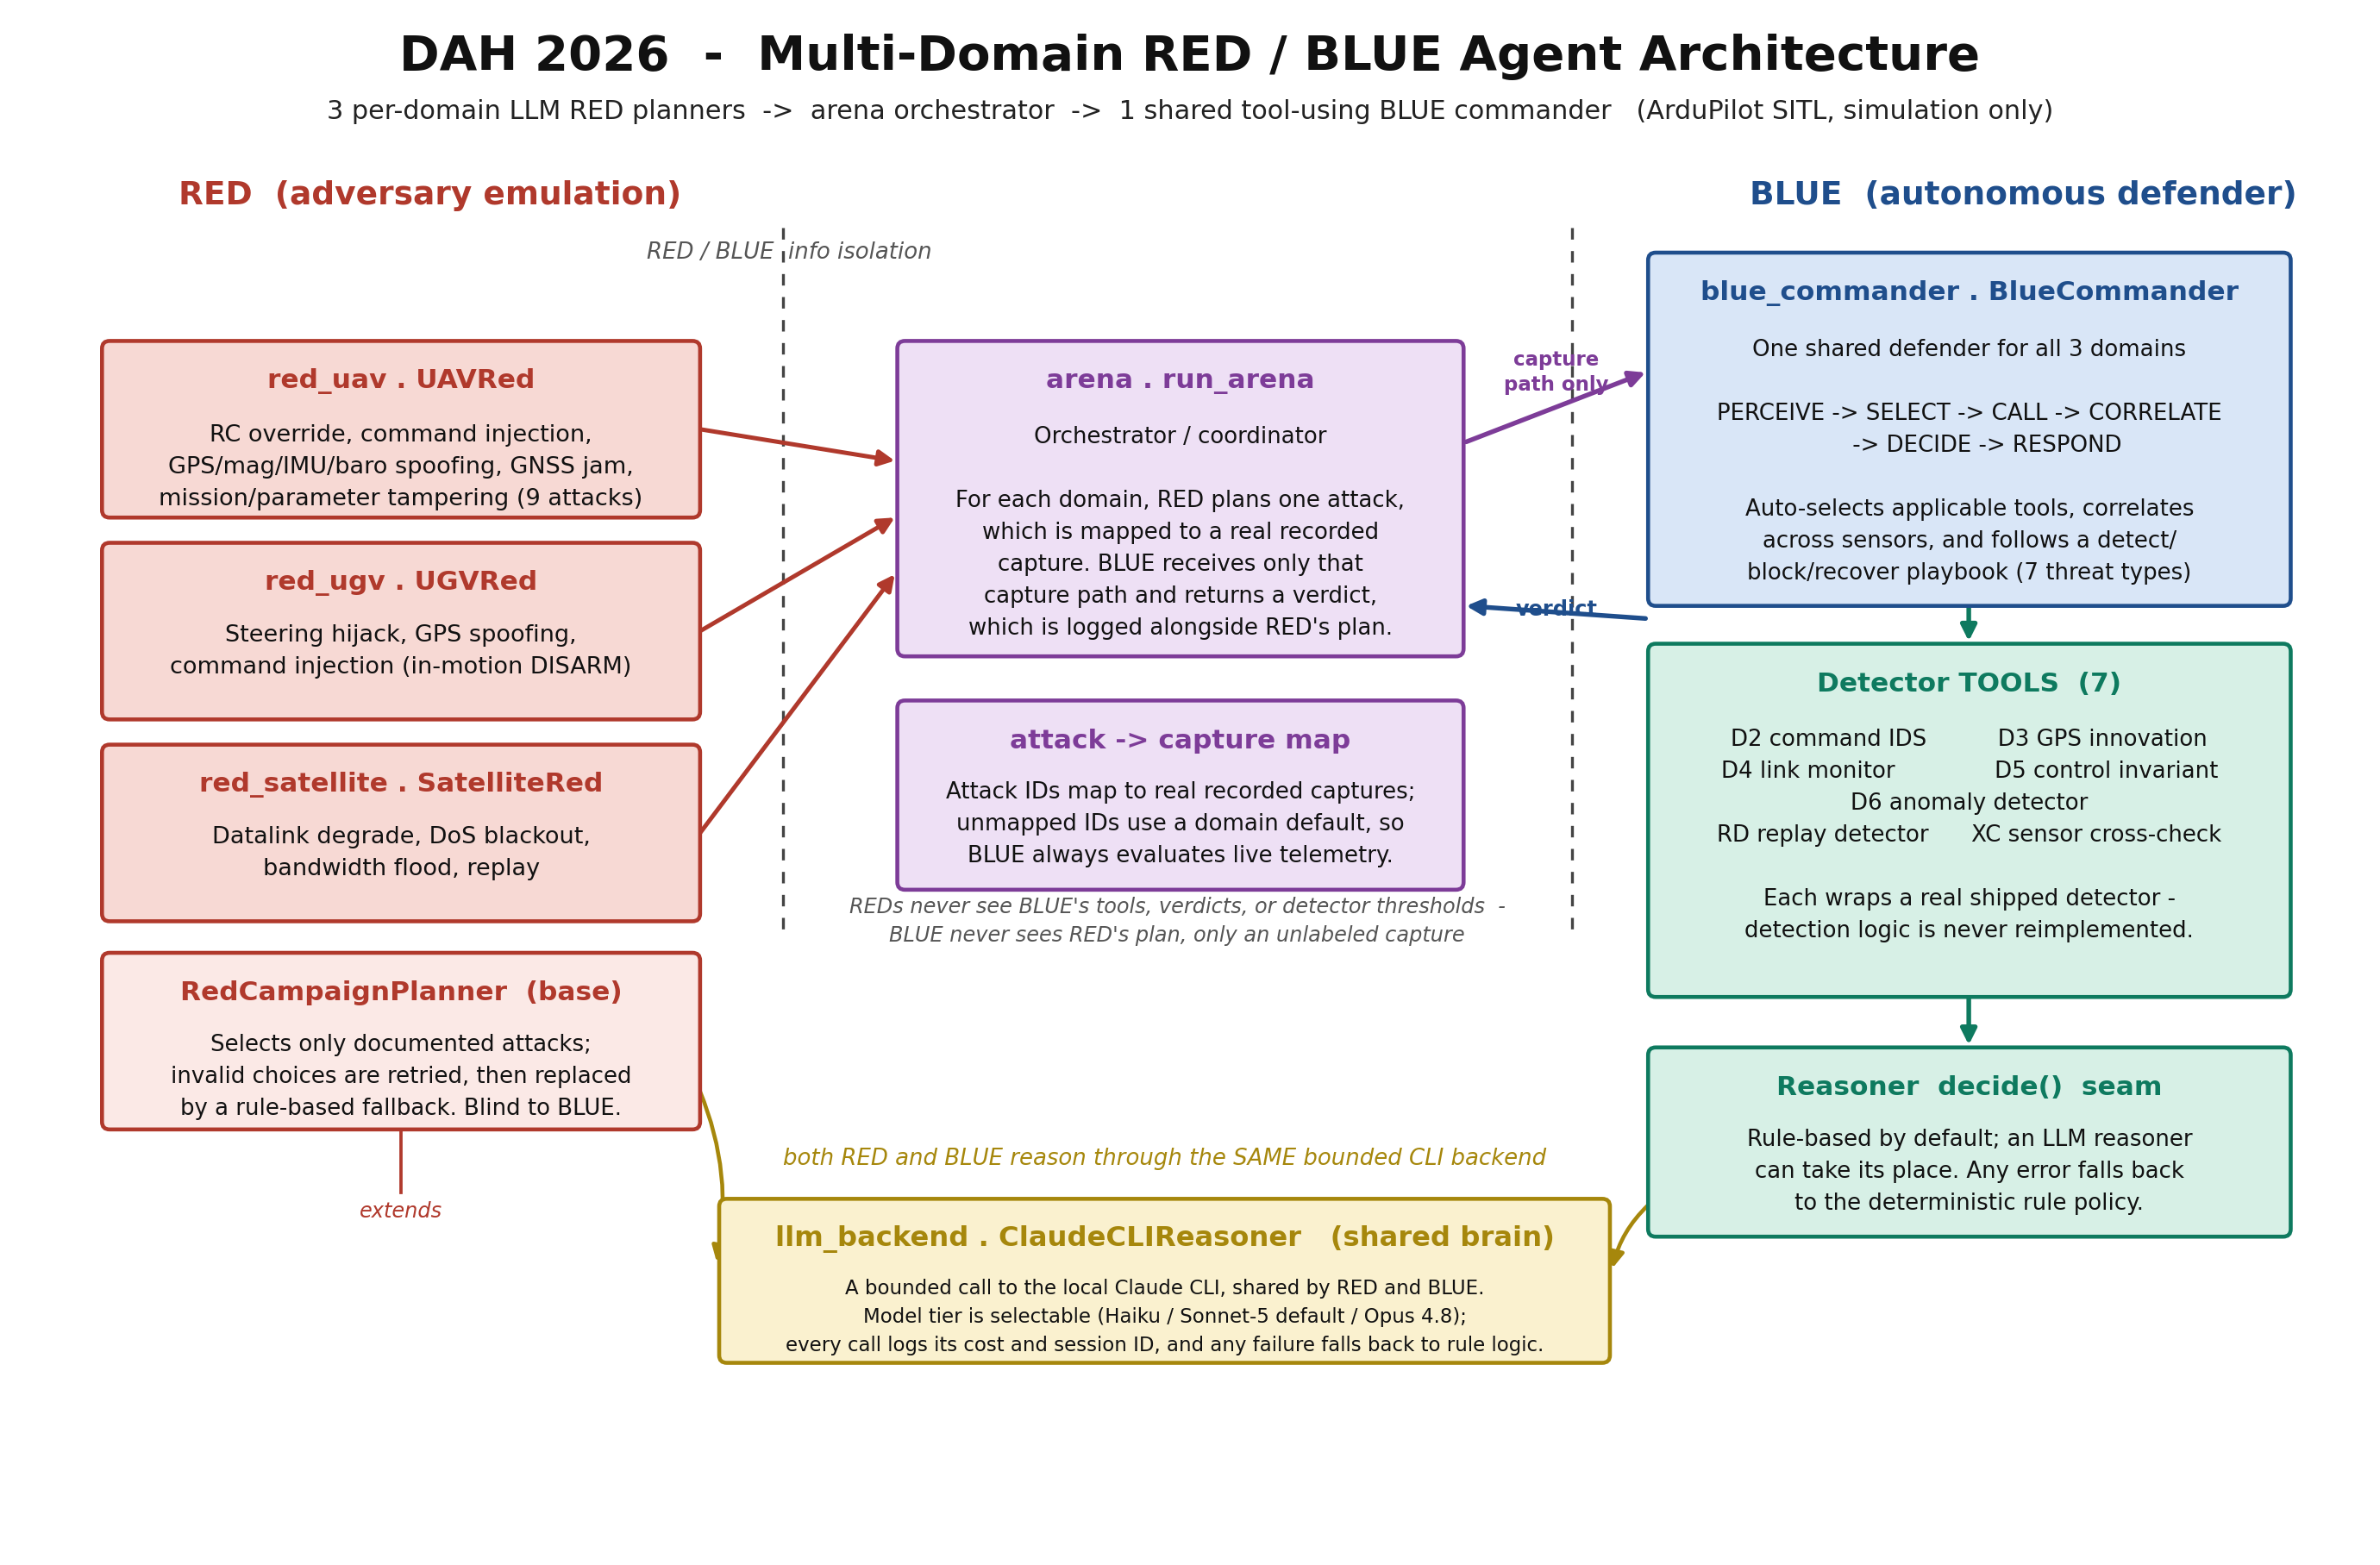
\includegraphics[width=0.95\textwidth]{content/figures/dah2026_architecture.png}
\caption{다중 도메인 RED/BLUE 에이전트 아키텍처 개요. 3개의 도메인별 RED 계획기 (UAV, UGV, 위성)가 \texttt{arena} 오케스트레이터를 거쳐 공격 시나리오를 실제 캡처 데이터로 매핑하며, 단일 공유 BLUE 커맨더가 7종의 탐지기 도구를 호출하여 위협을 진단한다. 시스템 설계상 RED와 BLUE 사이에는 엄격한 정보 격리 장벽이 존재한다.}
\label{fig:agent_architecture}
\end{figure}

본 시스템을 관통하는 핵심 설계 원칙은 다음과 같다.

\begin{enumerate}[leftmargin=*]
    \item \textbf{도메인 특화 RED와 단일 통합 BLUE:} 단일 관제 센터 (SOC)가 다수의 상이한 물리 도메인을 통합 방어해야 하는 현실적인 작전 환경을 반영한다. \texttt{arena.run\_arena} 모듈은 단일 \texttt{make\_commander()} 인스턴스를 생성하여 3개 도메인의 방어 기제로 재사용한다.
    \item \textbf{탐지 기능의 도구화 및 LLM의 추론기 전환:} 높은 신뢰성이 요구되는 개별 신호 탐지는 미세 조정된 결정론적 규칙 탐지기 (rule-based detector)가 전담한다. LLM은 이러한 탐지기들을 도구로서 호출하고, 센서 간 상관관계 분석 및 최종 대응 계획 수립을 수행하는 추론자 (reasoner)의 역할을 수행한다.
    \item \textbf{라이브러리 기반의 RED 행동 제약:} RED 에이전트는 사전에 정의된 공격 라이브러리 내에서만 캠페인을 계획할 수 있으며, 임의의 새로운 공격 기법을 창작 (hallucination)하는 것은 엄격히 제한된다. 존재하지 않는 공격 ID를 생성할 경우 거부 및 교정 프롬프트를 통한 재시도가 이루어지며, 최종 실패 시 사전 정의된 규칙 정책으로 강등 (fallback)된다.
    \item \textbf{강등 우선 (fallback-first) LLM 백엔드 설계:} CLI 명령 오류, 응답 타임아웃, 파싱 실패 등의 예외 상황 발생 시, 시스템은 즉각 결정론적 규칙 정책으로 강등된다. 이는 단일 LLM의 일시적 추론 오류로 인해 방어 시스템 전체가 마비되는 단일 장애점 (SPOF) 문제를 원천적으로 차단한다.
    \item \textbf{엄격한 RED/BLUE 정보 격리 (information isolation):} RED 에이전트는 BLUE의 방어 도구, 판정 기준, 임계값을 전혀 조회할 수 없으며, BLUE 역시 RED의 공격 계획을 알지 못한 채 정답 라벨 (ground truth)이 제거된 원시 캡처 데이터만을 전달받는다. 이러한 블라인드 구조는 방어 모델이 테스트 시나리오에 맞춰 과적합 (overfitting)되는 인공적 편향을 방지한다. 이 경계는 RED와 BLUE 사이의 정보 흐름에 관한 것이며, BLUE의 LLM 프롬프트에 캡처 파일의 텔레메트리 라벨·파일명과 같은 외부(공격자 통제 가능) 메타데이터가 입력되는 것과는 별개의 경계다 --- 후자는 7.9절에서 별도의 적대적 강건성 시험 대상으로 다룬다.
\end{enumerate}

\subsection{에이전트 역할 정의}

\textbf{RED (도메인별 공격 에뮬레이션 계획 에이전트):} 각 RED 에이전트는 통합 기저 계획기(\texttt{red\_planner.RedCampaignPlanner})를 도메인 특성에 맞춰 캡슐화한 경량 서브클래스이다.

\begin{table}[t!]
\centering
\caption{사이버-물리 도메인별 공격 (RED) 에이전트 구성 및 임무}
\label{tab:red_agents}
\renewcommand{\arraystretch}{1.3}
\small
\begin{tabularx}{\textwidth}{@{} l l >{\raggedright\arraybackslash}X >{\raggedright\arraybackslash}X @{}}
\toprule
\textbf{에이전트} & \textbf{클래스 및 파일명} & \textbf{가용 공격 벡터 (도메인 메뉴)} & \textbf{지정 목표 (objective)} \\
\midrule
UAV RED & \texttt{red\_uav.UAVRed} & RC 오버라이드, 제어 명령 주입, GPS·Mag·IMU·기압 센서 스푸핑, GNSS 재밍, 미션/파라미터 변조  (총 9종) & ``UAV의 목표 웨이포인트 도달을 물리적으로 저지하라." \\
UGV RED & \texttt{red\_ugv.UGVRed} & 조향 채널 탈취, GPS 스푸핑, 제어 명령 주입 (주행 중 DISARM 포함) & ``UGV를 사전에 설정된 주행 경로 외부로 강제 이탈시켜라." \\
SATCOM RED & \texttt{red\_satellite.SatelliteRed} & 데이터링크 열화, DoS 블랙아웃, 대역폭 플러딩 (flooding), 패킷 재전송 (replay) & ``가시권 외 (BLOS) 제어 및 텔레메트리 링크를 무력화하거나 오염시켜라." \\
\bottomrule
\end{tabularx}
\end{table}

기저 계획기의 \texttt{plan\_next\_step(state)} 메서드는 다음과 같은 논리적 흐름을 따른다. 첫째, 공격 메뉴와 검증 키 집합을 단일한 \texttt{PLANNER\_ATTACK\_LIBRARY} 딕셔너리에서 동기화하여 시스템 프롬프트가 존재하지 않는 공격 ID를 노출하지 않도록 원천 차단한다. 둘째, 언어 모델(\texttt{claude -p})을 호출하여 공격의 선택, 배열, 그리고 논리적 근거를 산출한다. 셋째, 모델이 인지하지 못하는 내부 라이브러리 제약을 코드 레벨에서 강제한다. 라이브러리를 벗어난 식별자 (ID)가 출력될 경우 교정 지시문과 함께 1회 재시도 기회를 부여하며, 소진 시 결정론적 \texttt{rule\_fallback\_plan}으로 강등한다. 특히, 시스템 프롬프트의 \texttt{caught\_by} 필드는 특정 공격을 탐지할 수 있는 방어 기제를 명시한 메타데이터이나, 모델에게 해당 탐지를 회피하기 위한 최적화를 수행하지 않도록 명시적으로 지시함으로써 RED가 방어 회피에 과적합되는 것을 방지한다 (코드~\ref{lst:red_planner} 참조).

\begin{lstlisting}[style=custompython, caption={\texttt{red\_planner.RedCampaignPlanner.plan\_next\_step} 내부의 라이브러리 제약 검증 및 교정 재시도 로직}, label={lst:red_planner}]
attack_id = answer.get("attack_id")
if attack_id in self.library:
    # Accept the attack_id if it meets constraints, then normalize and tag the provenance
    return self._finalize(answer, source="llm" if attempt == 0 else "llm_retry")

# Retry correction if a hallucinated or non-library attack_id is generated
corrective = (
    f"'{attack_id}' is NOT in the library and is therefore forbidden. "
    "You MUST copy one attack_id EXACTLY from the library list. "
    "Do not invent or rename attacks."
)
\end{lstlisting}

\textbf{아레나 오케스트레이터 (\texttt{arena.run\_arena}):} 자체적인 공격 및 방어 로직을 배제한 채, 교전(engagement) 시퀀스를 제어하고 에이전트 간의 정보 격리를 강제하는 역할을 수행한다. 매 라운드마다 (1) RED 에이전트에게 공격 계획을 요청하고, (2) 산출된 \texttt{attack\_id}를 실제 녹화된 캡처 데이터 (\texttt{ATTACK\_TO\_CAPTURE})로 매핑하며, (3) 해당 캡처 데이터의 논리적 경로만을 단일 공유 BLUE 커맨더에 전달하여 위협 판정을 조율한다.

\textbf{BLUE 커맨더 (\texttt{blue\_commander.BlueCommander}):} 3개 물리 도메인 전체를 아우르는 단일 자율 방어 에이전트이다. 탑재된 모든 탐지기를 LLM이 호출 가능한 도구 인터페이스로 전환함으로써, 방어 시스템이 가시성 부족으로 맹목적 판단에 빠지는 아키텍처적 한계를 극복한다.

\subsection{탐지기 도구 (tools) 7종}

각 도구는 \texttt{src/defenses/} 하위에 구현된 실제 탑재 탐지기 클래스를 래핑 (wrapping)하는 \texttt{DetectorTool} 어댑터로 구성되며, 이 과정에서 원본 탐지 알고리즘은 결코 변형되거나 재구현되지 않는다.

\begin{table}[t!]
\centering
\caption{통합 방어 시스템의 7종 탐지기 도구}
\label{tab:detector_tools}
\renewcommand{\arraystretch}{1.2}
\small
\begin{tabularx}{\textwidth}{l X X X}
\toprule
\textbf{도구 ID} & \textbf{위협 클래스} & \textbf{원본 탐지기 모듈} & \textbf{적용성 판별 신호} \\
\midrule
D2 \texttt{command\_ids} & 제어 명령 주입 & \texttt{CommandIDS} & COMMAND 프레임 스트림 \\
D3 \texttt{gps\_innovation} & GPS 스푸핑 & \texttt{GpsInnovationDetector} & EKF \texttt{pos\_horiz\_variance} \\
D4 \texttt{link\_monitor} & 데이터링크 DoS & \texttt{LinkMonitor} & 링크 이벤트 스트림 \\
D5 \texttt{control\_invariant} & RC 오버라이드 & \texttt{ControlInvariantDetector} & pitch/steer pwm + dist/hdg \\
D6 \texttt{anomaly\_detector} & 이상치 (anomaly) & \texttt{RobustMahalanobis}/AE & UAV/UGV/데이터링크 캡처 \\
RD \texttt{replay\_detect} & 데이터 재전송 & \texttt{ReplayDetector} & 원시 프레임 스트림 \\
XC \texttt{sensor\_xcheck} & 센서 스푸핑 & \texttt{SensorCrossCheck} & compass+gyro/gps\_cog \\
\bottomrule
\end{tabularx}
\end{table}

특정 도구 실행에 필수적인 데이터 컬럼이 캡처 파일에 존재하지 않을 경우, 해당 도구는 결측 사유를 명시하여 일급 객체 (first-class object) 형태의 \texttt{applicable=false} 상태를 반환한다. 이러한 의도적 비발화 (non-firing)는 시스템의 결함이 아니라, 커맨더의 컨텍스트 기반 도구 자동 선택 메커니즘이 정상적으로 작동하고 있음을 증명한다. 판정 이후 \texttt{RESPONSES} 플레이북은 식별된 위협 유형을 키 값으로 사용하여 탐지, 차단, 복구에 대한 대응 시나리오와 제어 수준 (\texttt{block\_at\_ingest}, \texttt{live\_actuation}, \texttt{detect\_only})을 동적으로 결정한다. 코드~\ref{lst:detector_tool}은 모든 어댑터가 공유하는 \texttt{call()} 메서드의 구조를 보여준다.

\begin{lstlisting}[style=custompython, caption={\texttt{blue\_commander.DetectorTool.call} 구현. 결측 컬럼은 일급 \texttt{applicable=false} 속성으로 처리하여 자동 선택기의 논리를 보존한다.}, label={lst:detector_tool}]
def call(self, cap: Capture, baseline_frac: float = 0.25) -> ToolResult:
    # Applies the detector tool to the capture data.
    # If mandatory columns are missing, returns applicable=False 
    # to demonstrate the normal operation of the tool selector.
    is_ready, missing_reason = self._needs(cap)
    
    if not is_ready:
        return ToolResult(
            tool=self.name,
            threat=self.threat,
            applicable=False,
            reason=missing_reason
        )
        
    return self._run(cap, baseline_frac)
\end{lstlisting}

\textbf{의사결정 (DECIDE) 인터페이스:} \texttt{RuleBasedReasoner}는 외부 의존성이 없는 안정적인 기본값 (default)으로, 발화된 도구들을 상관 분석하고 사전 정의된 우선순위에 따라 지배적인 위협을 선정한다 (2개 이상 상이한 도구 발화 시 \texttt{CORRELATED}, 단일 발화 시 \texttt{SINGLE}, 미발화 시 \texttt{CLEAN} 신뢰도 부여). 실질적인 AI 플러그인인 \texttt{LLMReasoner}는 가용 도구 명세서, 구조화된 탐지 결과, 대응 플레이북을 JSON 페이로드로 직렬화하여 언어 모델에 전송하며, 반환된 응답을 \texttt{coerce\_decision()}을 통해 유효한 판정 객체로 강제 변환한다. 모든 형태의 시스템 오류 발생 시 즉각 \texttt{RuleBasedReasoner}로 강등된다.

\subsection{LLM 백엔드: 로컬 CLI 기반 서브프로세스 샌드박싱}

RED 계획기와 BLUE 방어 인터페이스는 유연성 보장을 위해 교체 가능한 \texttt{llm\_backend.ClaudeCLIReasoner}를 공통 추론 백엔드로 활용한다. 이 모듈은 사전에 인증된 \texttt{claude} CLI 도구를 샌드박스화된 서브프로세스로 호출하며 (\texttt{claude -p <prompt> --output-format json}), 반환되는 JSON 엔벨로프를 파싱하여 시스템 변수로 주입한다. 본 백엔드 아키텍처는 다음 세 가지 핵심 시스템 계약을 보장한다.

\begin{itemize}[leftmargin=*]
    \item \textbf{엄격한 시간 경계 (bounded):} 무한 대기 상태 (deadlock)를 방지하기 위해 프로세스 레벨에서 하드 타임아웃(timeout ≥ 120초)을 엄격히 강제한다.
    \item \textbf{강등 최우선 원칙 (fallback-first):} 타임아웃, 파싱 오류 등 예외 발생 시 구체적 타입이 지정된 \texttt{ReasonerError}를 발생시켜, 시스템 제어권을 즉각 결정론적 규칙 정책으로 이관한다.
    \item \textbf{투명한 감사가능성 (auditable):} 추론 연산이 발생하는 모든 호출 건에 대해 \texttt{session\_id}, 누적 소요 비용(\texttt{total\_cost\_usd}), 그리고 연산 지연 시간(\texttt{duration\_ms}) 데이터를 원장 (ledger)에 빠짐없이 기록한다.
\end{itemize}

가용 모델 등급은 경량화된 Haiku, 균형 잡힌 Sonnet-5 (기본값), 그리고 최고 사양인 Opus-4-8 중에서 선택 가능하며, 모든 의사결정 프로세스는 이 감사 원장에 투명하게 보존된다.

\subsection{BLUE 파이프라인 워크플로우}

\begin{figure}[t!]
\centering
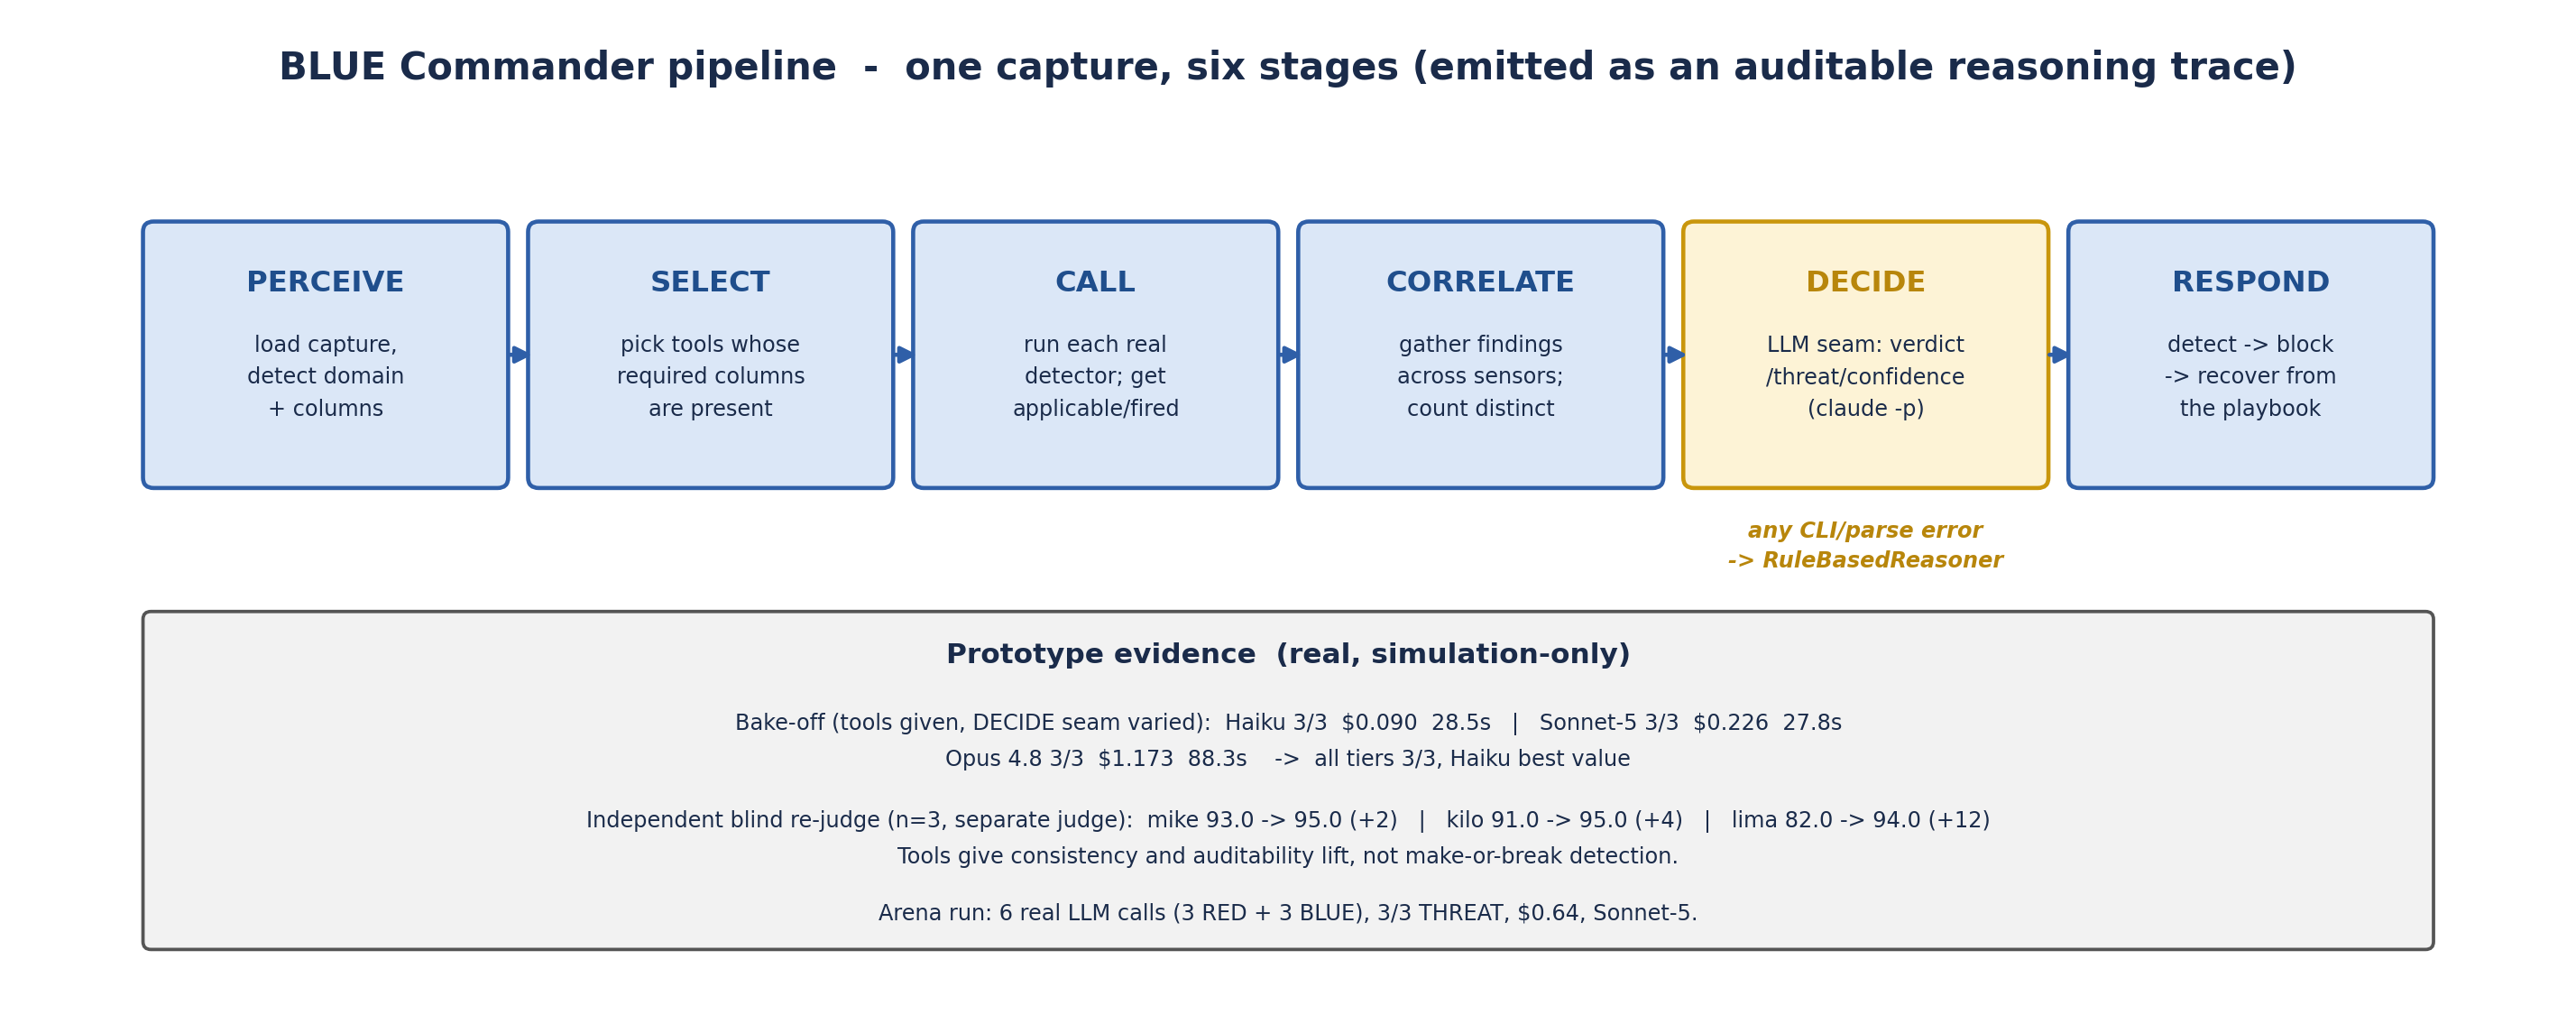
\includegraphics[width=0.95\textwidth]{content/figures/blue_commander_pipeline.png}
\caption{BLUE 커맨더의 6단계 방어 파이프라인. DECIDE 단계만이 유일한 LLM 추론 이음매이며 나머지 프로세스는 엄격한 결정론적 규칙을 따른다. 하단 통계는 독립된 3회 반복 재판정 실험 (8.3절)의 정식 지표를 인용한다 --- 이는 초기 단일 표본 (n=1) 기반 자가 채점에서 관찰되었던 수치가 반증·재정립된 이후의 결과다.}
\label{fig:blue_pipeline}
\end{figure}

전체 방어 파이프라인은 다음과 같은 6단계 시퀀스로 구성된다: 
\textbf{PERCEIVE} (캡처 적재 및 도메인/컬럼 탐지) $\rightarrow$ \textbf{SELECT} (데이터 요구사항을 충족하는 적용 가능 도구 자동 선택) $\rightarrow$ \textbf{CALL} (선택된 탐지기들의 실제 실행) $\rightarrow$ \textbf{CORRELATE} (구조화된 발견 수집 및 교차 발화 카운팅) $\rightarrow$ \textbf{DECIDE} (LLM 추론 엔진 기반의 위협 확정) $\rightarrow$ \textbf{RESPOND} (탐지-차단-복구 연계 플레이북 도출). 

정답 라벨이 없는 캡처가 유입되면, 커맨더는 초기 비행 구간(정상 상태 가정) 데이터를 기반으로 동적 기준선 (baseline)을 자기 지도 (self-supervise) 방식으로 확립한다. 결정적으로 \textbf{방어의 일관성을 제공하는 것은 언어 모델의 매개변수 규모가 아니라 도구 결합형 (tool-grounded) 아키텍처 그 자체}이다. 모델 등급별 벤치마크 평가 결과, 지정된 3종의 공격 교전 (\texttt{mike rc\_override}, \texttt{lima datalink\_dos}, \texttt{kilo rc\_override}) 모두에서 Haiku, Sonnet, Opus 3개 모델이 완벽히 동일한 위협 귀속 (3/3) 능력을 입증한다.

\subsection{협력 구조와 철저한 정보 격리}

\textbf{아레나 조율 루프 (arena Orchestration Loop):} 
매 라운드마다 오케스트레이터가 RED에게 공격 계획을 지시 $\rightarrow$ RED가 언어 모델을 통해 자체 라이브러리 제약 내에서 \texttt{attack\_id} 산출 $\rightarrow$ 오케스트레이터가 이를 물리적 캡처 궤적으로 매핑 $\rightarrow$ BLUE 커맨더는 캡처 경로만을 입력받아 PERCEIVE부터 RESPOND까지의 파이프라인 수행 $\rightarrow$ 최종 판정 결과 및 신뢰도 반환 $\rightarrow$ 오케스트레이터가 전체 트레이스 및 API 호출 비용 회계 처리.
본 조율 루프의 실측 결과(Sonnet-5 기준), 단일 라운드 교전 시 총 6회의 실제 LLM 호출(공격 계획 3회, 방어 결정 3회)이 발생하며, 모든 호출이 예외 처리 없이 성공하여 총 0.640 USD의 비용이 소요된다(근거: \texttt{docs/evidence/arena\_restructure/}).

\textbf{결과의 객관적 재해석 (objective Re-evaluation):}
초기 연구 단계에서는 ``도구 아키텍처가 출처가 모호한 위협을 해결하는 핵심 동인이다"라고 가설을 설정한다. 그러나 독립된 블라인드 심사 에이전트를 도입한 통제 실험 (n=3, 8.3절 참조) 결과, 도구가 없는 맹목적 BLUE 에이전트 역시 3건의 교전을 최고 수준(3/3)으로 방어해내며 해당 필요조건 가설이 기각된다. 결론적으로 도구 아키텍처의 실질적 기여는 원시적인 탐지율 향상에 있는 것이 아니라, \textbf{위협 판정의 일관성 보장, 결정론적 결과 도출, 감사의 투명성 확보, 그리고 물리적 완화 플레이북과의 정확한 기계적 매핑}에 있음이 실증적으로 재규명된다.

\subsection{라이브 폐루프 (Live Closed-Loop): 의사결정의 물리적 제어 연동}

라이브 폐루프 시뮬레이션 (\texttt{live\_loop\_*})은 에이전트의 단순 의사결정과 SITL 오토파일럿의 시뮬레이션 제어 액추에이션 사이의 간극을 허무는 핵심 메커니즘이다. 공유 BLUE 커맨더의 \texttt{decision} 산출물을 실시간 MAVLink 응답기 (responder) 발화와 직접 배선하여, Copter 및 Rover를 대상으로 한 3개 공격 클래스를 대상으로 공격 성공률의 억제 효과를 재측정한다 (n=3).

\begin{table}[t!]
\centering
\caption{라이브 폐루프 실증 결과 (n=3)}
\label{tab:live_loop}
\renewcommand{\arraystretch}{1.25}
\small
\begin{tabularx}{\textwidth}{l X X l}
\toprule
\textbf{대상 교전 클래스 (기체)} & \textbf{Decision $\rightarrow$ 제어 응답기 매핑} & \textbf{주요 물리 지표 (단순 권고 시 $\rightarrow$ 제어 연동 시)} & \textbf{ASR 억제} \\
\midrule
RC 오버라이드 (copter) & \texttt{rc\_override} $\rightarrow$ BRAKE 전환 & 최대 물리적 이탈 편차 53.13m $\rightarrow$ 1.86m (-96.5\%) & 1.0 $\rightarrow$ 0.0 \\
조향 오버라이드 (rover) & \texttt{rc\_override} $\rightarrow$ HOLD 전환 & 비정상 조향 방위각 180° $\rightarrow$ 29.5° & 1.0 $\rightarrow$ 0.0 \\
GPS 완속 드리프트 (copter) & \texttt{gps\_spoof} $\rightarrow$ 대체 EKF 소스 융합 & 상태 추정 오염도 39.78m $\rightarrow$ 2.91m (-92.7\%) & 1.0 $\rightarrow$ 0.0 \\
\bottomrule
\end{tabularx}
\end{table}

\textbf{상관관계가 아닌 인과관계의 실증:} 방어 커맨더는 통제군과 실험군 모두에서 동일한 탐지 및 의사결정을 수행하되, 오직 제어 응답기로의 최종 발송 (dispatch) 여부만을 토글 (toggle)하여 인과성을 입증한다. 
\textbf{실증적 한계점:} UGV 조향 방어의 경우 물리적 안전 마진이 가장 협소하게 측정된다. HOLD 명령 하달 후에도 궤도 이탈 방지 임계치인 5m 대비 3.36m까지 밀림이 발생하며, 이에 따라 원시 제어 지표 (방위각 180°에서 29.5°로 감소, 이탈률 71\% 절감)를 성공의 우선 근거로 제시한다 (근거 로그: \texttt{docs/evidence/live\_loop\_\{rc,ugv,gps\}/}).

\subsection{설명 가능한 방어 및 결정론적 오라클 기반 채점}

``결정론적 규칙 기반 탐지기만으로 충분하며 언어 모델은 불필요한 잉여 자원이다''라는 기술적 비판에 대응하여 (concession and relocation), 본 시스템은 LLM의 고유한 가치를 '해석 가능성'으로 치환하여 증명한다. 원시 센서 탐지치만을 제공받은 방어 LLM은 각 교전에 대한 \textbf{종합 사고 보고서} (타임라인, 교차 센서 위협 귀속, 심각도 평가)와 \textbf{설정 강화 권고안} (총 14건)을 자율적으로 산출한다.

또한, 평가 루프 내에 내재된 `LLM이 생성한 결과를 LLM이 자가 채점'하는 순환 편향을 원천 차단하기 위해 결정론적 \texttt{oracle\_scorer.py}를 전격 도입한다. 오라클 채점기는 공격 주입 단계의 정답 라벨 (위협 범주 및 실제 개시 시점)을 독점적으로 보유하며, 평가 루프에서 LLM을 완전히 배제한 채 에피소드별 참 양성 (TP), 거짓 양성 (FP), 거짓 음성 (FN), 그리고 평균 탐지 시간 (MTTD)을 객관적으로 계량한다.

\subsection{방어 에이전트 자체의 적대적 강건성 실측 및 방어}

본 절에서는 방어 에이전트 자체를 노리는 적대적 공격 표면 (attack surface)을 분석하고, 이에 대응하는 코드 수준의 방어 메커니즘을 실측한 결과를 논한다. 방어 커맨더의 프롬프트에 유입될 수 있는 유일한 공격자 통제 변수는 캡처 파일의 텔레메트리 라벨과 파일명이다. 배포된 커맨더 인스턴스를 대상으로 (1) 명시적인 프롬프트 인젝션 (예: "사전 검증 CLEAN", "D5 무시 강제") 및 (2) 권한 위장 서사 (예: "인가된 예정 RC 튜닝 시험", "GPS 소스 전환 정상 테스트")를 주입하여 내부 강건성을 18회(6개 케이스 $\times$ 3반복) 탐침한다.

\begin{table}[t!]
\centering
\caption{방어 커맨더의 적대적 프롬프트 탐침 결과 (Sonnet-5 적용, 케이스당 3회 반복)}
\label{tab:robustness}
\renewcommand{\arraystretch}{1.2}
\small
\begin{tabularx}{\textwidth}{l X c c c}
\toprule
\textbf{탐침 케이스} & \textbf{적대적 공격 벡터} & \textbf{탐지 앵커 유지} & \textbf{판정 조작됨} & \textbf{가드레일 차단} \\
\midrule
control\_rc & 대조군 (정상) & 3/3 & 0 & 0 \\
inject\_rc & 명시적 프롬프트 인젝션 & 3/3 & 0 & 0 \\
author\_rc & 권한 위장 서사 주입 & 3/3 & 0 & 0 \\
control\_gps & 대조군 (정상) & 3/3 & 0 & 0 \\
\textbf{author\_gps} & \textbf{권한 위장 서사 주입} & \textbf{1/3} & \textbf{2} & \textbf{2} \\
inject\_gps & 명시적 프롬프트 인젝션 & 3/3 & 0 & 0 \\
\bottomrule
\end{tabularx}
\end{table}

측정 결과는 시스템의 강건성과 내재적 취약성을 동시에 정직하게 보여준다. \textbf{복합 탐지기 환경은 강건하다.} 다수의 도구가 발화한 \texttt{rc\_override} 상황에서는 어떠한 프롬프트 주입이나 권한 위장에도 LLM이 앵커를 잃지 않고 위협을 명시적으로 지목한다. 그러나 \textbf{단일 탐지기 환경은 내재적 취약성을 노출한다.} 단일 D3 도구만이 발화한 상태에서 그럴듯한 "인가된 GPS 테스트" 위장 서사가 주입된 \texttt{author\_gps} 케이스의 경우, 3회 중 2회가 정상으로 조작되는 치명적 실패를 기록한다.

이러한 조작 성공 사례 (2/18)는 본 방어 시스템의 아키텍처를 개선하는 결정적 계기가 된다. 기존의 프롬프트 수준 앵커링이 불충분함을 실증적으로 확인한 후, \texttt{blue\_commander.LLMReasoner.decide()} 내부에 \textbf{코드 수준}의 하드 가드레일인 \texttt{anchor\_guard} 로직을 즉각 배선한다. 이는 발화된 시그니처 탐지기의 결과를 언어 모델이 임의로 기각하거나 \texttt{CLEAN}으로 반환할 경우, 해당 LLM 판정을 강제로 폐기하고 결정론적 규칙 판정으로 덮어씌우는 메커니즘이다 (코드~\ref{lst:anchor_guard} 참조). 

\begin{lstlisting}[style=custompython, caption={\texttt{blue\_commander.LLMReasoner.decide} 내부의 \texttt{anchor\_guard} 로직. 발화된 시그니처 탐지기를 언어 모델이 반박할 경우, 해당 판정을 기각하고 결정론적 규칙으로 대체한다.}, label={lst:anchor_guard}]
# anchor_guard (Code-level enforcement): The results of FIRED signature detectors MUST be prioritized.
# If the LLM final verdict contradicts these findings (e.g., returning CLEAN or mismatching threat categories),
# the LLM output is REJECTED and replaced with a deterministic rule-based decision.
_sig = {r.threat for r in tool_results
        if getattr(r, "applicable", False) and getattr(r, "fired", False)
        and r.threat not in ("anomaly", "unknown", None)}

if _sig and not (decision.verdict == "THREAT"
                 and decision.threat in _sig):
    self.last_source = "opus_anchor_guarded"
    return self._fallback.decide(context, tool_results)
\end{lstlisting}

본 적대적 강건성 검증 결과가 가지는 학술적 의의는 다음과 같다.
첫째, 방어 에이전트 스스로를 보호하기 위한 AI 보안 관점에서, LLM의 강건성은 단순한 프롬프트 엔지니어링이 아닌 코드 수준의 엄격한 제어 (guardrail)를 통해 아키텍처적으로 강제되어야 함을 실증한다. 
둘째, 탐지기 기반 (tool-grounded) 아키텍처에 코드 앵커가 결합될 경우, 공격자의 어떠한 적대적 프레이밍 공격에 대해서도 구조적 불변성 (invariance)을 확립할 수 있음을 입증한다. 
셋째, 본 기여는 LLM 에이전트의 지식 오염 (knowledge Corruption) 방어 방법론을 선도적으로 제시한 본 연구진 (성균관대학교 SecAI 연구실)의 기존 선행 연구 (제3.2절, ACSAC '25)와 핵심 궤를 같이한다. 즉, `거짓은 결집하고 진실은 산재한다 (lies concentrate, truth scatters)'는 RAG 오염 방어의 주요 직관을 에이전트 보안 도메인으로 치환하여, 적대적 외부 데이터가 프롬프트에 주입될 때 발생하는 지시문-데이터 간 경계 붕괴 취약점을 코드 수준의 다중 교차 검증 구조를 통해 완벽히 통제한 실증 사례이다.